\documentclass{article}
\usepackage{graphicx}
\usepackage{xcolor}
\usepackage{amsfonts}
\usepackage{amsmath}
\usepackage{geometry}
\usepackage{caption}
\usepackage{subcaption}
\usepackage[framemethod=TikZ]{mdframed}
\usepackage{amsthm}
\usepackage{enumerate}
\usepackage{soul}
\sethlcolor{pink}

%%%%%%%%%%%%%%%%%%%%%%%%%%%%%%
%Theorem
\newcounter{theo}[section] \setcounter{theo}{0}
\renewcommand{\thetheo}{\arabic{section}.\arabic{theo}}
\newenvironment{theo}[2][]{%
	\refstepcounter{theo}%
	\ifstrempty{#1}%
	{\mdfsetup{%
			frametitle={%
				\tikz[baseline=(current bounding box.east),outer sep=0pt]
				\node[anchor=east,rectangle,fill=blue!20]
				{\strut Theorem~\thetheo};}}
	}%
	{\mdfsetup{%
			frametitle={%
				\tikz[baseline=(current bounding box.east),outer sep=0pt]
				\node[anchor=east,rectangle,fill=blue!20]
				{\strut Theorem~\thetheo:~#1};}}%
	}%
	\mdfsetup{innertopmargin=10pt,linecolor=blue!20,%
		linewidth=2pt,topline=true,%
		frametitleaboveskip=\dimexpr-\ht\strutbox\relax
	}
	\begin{mdframed}[]\relax%
		\label{#2}}{\end{mdframed}}
%%%%%%%%%%%%%%%%%%%%%%%%%%%%%%
%Lemma
\newcounter{lem}[section] \setcounter{lem}{0}
\renewcommand{\thelem}{\arabic{section}.\arabic{lem}}
\newenvironment{lem}[2][]{%
	\refstepcounter{lem}%
	\ifstrempty{#1}%
	{\mdfsetup{%
			frametitle={%
				\tikz[baseline=(current bounding box.east),outer sep=0pt]
				\node[anchor=east,rectangle,fill=green!20]
				{\strut Lemma~\thelem};}}
	}%
	{\mdfsetup{%
			frametitle={%
				\tikz[baseline=(current bounding box.east),outer sep=0pt]
				\node[anchor=east,rectangle,fill=green!20]
				{\strut Lemma~\thelem:~#1};}}%
	}%
	\mdfsetup{innertopmargin=10pt,linecolor=green!20,%
		linewidth=2pt,topline=true,%
		frametitleaboveskip=\dimexpr-\ht\strutbox\relax
	}
	\begin{mdframed}[]\relax%
		\label{#2}}{\end{mdframed}}
%%%%%%%%%%%%%%%%%%%%%%%%%%%%%%
%Proof
\newcounter{prf}[section]\setcounter{prf}{0}
\renewcommand{\theprf}{\arabic{section}.\arabic{prf}}
\newenvironment{prf}[2][]{%
	\refstepcounter{prf}%
	\ifstrempty{#1}%
	{\mdfsetup{%
			frametitle={%
				\tikz[baseline=(current bounding box.east),outer sep=0pt]
				\node[anchor=east,rectangle,fill=red!20]
				{\strut Proof~\theprf};}}
	}%
	{\mdfsetup{%
			frametitle={%
				\tikz[baseline=(current bounding box.east),outer sep=0pt]
				\node[anchor=east,rectangle,fill=red!20]
				{\strut Proof~\theprf:~#1};}}%
	}%
	\mdfsetup{innertopmargin=10pt,linecolor=red!20,%
		linewidth=2pt,topline=true,%
		frametitleaboveskip=\dimexpr-\ht\strutbox\relax
	}
	\begin{mdframed}[]\relax%
		\label{#2}}{\qed\end{mdframed}}
%%%%%%%%%%%%%%%%%%%%%%%%%%%%%%
%Highlight
\newcounter{imp}[section]\setcounter{imp}{0}
\renewcommand{\theimp}{\arabic{section}.\arabic{imp}}
\newenvironment{imp}[2][]{%
	\refstepcounter{imp}%
	\ifstrempty{#1}%
	{\mdfsetup{%
			frametitle={%
				\tikz[baseline=(current bounding box.east),outer sep=0pt]
				\node[anchor=east,rectangle,fill=yellow!20]
				{\strut ~\theimp};}}
	}%
	{\mdfsetup{%
			frametitle={%
				\tikz[baseline=(current bounding box.east),outer sep=0pt]
				\node[anchor=east,rectangle,fill=yellow!20]
				{\strut ~\theimp:~#1};}}%
	}%
	\mdfsetup{innertopmargin=10pt,linecolor=yellow!20,%
		linewidth=2pt,topline=true,%
		frametitleaboveskip=\dimexpr-\ht\strutbox\relax
	}
	\begin{mdframed}[]\relax%
		\label{#2}}{\end{mdframed}}
%%%%%%%%%%%%%%%%%%%%%%%%%%%%%%
%Example
\newcounter{example}[section]\setcounter{example}{0}
\renewcommand{\theexample}{\arabic{section}.\arabic{example}}
\newenvironment{example}[2][]{%
	\refstepcounter{example}%
	\ifstrempty{#1}%
	{\mdfsetup{%
			frametitle={%
				\tikz[baseline=(current bounding box.east),outer sep=0pt]
				\node[anchor=east,rectangle,fill=purple!20]
				{\strut Example~\theexample};}}
	}%
	{\mdfsetup{%
			frametitle={%
				\tikz[baseline=(current bounding box.east),outer sep=0pt]
				\node[anchor=east,rectangle,fill=purple!20]
				{\strut Example~\theexample:~#1};}}%
	}%
	\mdfsetup{innertopmargin=10pt,linecolor=red!20,%
		linewidth=2pt,topline=true,%
		frametitleaboveskip=\dimexpr-\ht\strutbox\relax
	}
	\begin{mdframed}[]\relax%
		\label{#2}}{\end{mdframed}}
%%%%%%%%%%%%%%%%%%%%%%%%%%%%%%
%Definition
\newcounter{defn}[section]\setcounter{defn}{0}
\renewcommand{\thedefn}{\arabic{section}.\arabic{defn}}
\newenvironment{defn}[2][]{%
	\refstepcounter{defn}%
	\ifstrempty{#1}%
	{\mdfsetup{%
			frametitle={%
				\tikz[baseline=(current bounding box.east),outer sep=0pt]
				\node[anchor=east,rectangle,fill=purple!20]
				{\strut Definition~\thedefn};}}
	}%
	{\mdfsetup{%
			frametitle={%
				\tikz[baseline=(current bounding box.east),outer sep=0pt]
				\node[anchor=east,rectangle,fill=purple!20]
				{\strut Definition~\thedefn:~#1};}}%
	}%
	\mdfsetup{innertopmargin=10pt,linecolor=red!20,%
		linewidth=2pt,topline=true,%
		frametitleaboveskip=\dimexpr-\ht\strutbox\relax
	}
	\begin{mdframed}[]\relax%
		\label{#2}}{\end{mdframed}}
%%%%%%%%%%%%%%%%%%%%%%%%%%%%%%
%Exercise
\newcounter{exer}[section]\setcounter{exer}{0}
\renewcommand{\theexer}{\arabic{section}.\arabic{exer}}
\newenvironment{exer}[2][]{%
	\refstepcounter{exer}%
	\ifstrempty{#1}%
	{\mdfsetup{%
			frametitle={%
				\tikz[baseline=(current bounding box.east),outer sep=0pt]
				\node[anchor=east,rectangle,fill=lightgray!20]
				{\strut Exercise~\theexer};}}
	}%
	{\mdfsetup{%
			frametitle={%
				\tikz[baseline=(current bounding box.east),outer sep=0pt]
				\node[anchor=east,rectangle,fill=lightgray!20]
				{\strut Exercise~\theexer:~#1};}}%
	}%
	\mdfsetup{innertopmargin=10pt,linecolor=lightgray!20,%
		linewidth=2pt,topline=true,%
		frametitleaboveskip=\dimexpr-\ht\strutbox\relax
	}
	\begin{mdframed}[]\relax%
		\label{#2}}{\end{mdframed}}
%%%%%%%%%%%%%%%%%%%%%%%%%%%%%%



\DeclareMathOperator{\bX}{\boldsymbol{X}}
\DeclareMathOperator{\iid}{\stackrel{iid}{\sim}}
\DeclareMathOperator{\hbb}{\hat{\boldsymbol{\beta}}}
\DeclareMathOperator{\bY}{\boldsymbol{Y}}
\DeclareMathOperator{\bH}{\boldsymbol{H}}
\DeclareMathOperator{\hbmu}{\hat{\boldsymbol{\mu}}}
\DeclareMathOperator{\bmu}{\boldsymbol{\mu}}
\DeclareMathOperator{\real}{\mathbb{R}}
\DeclareMathOperator{\bP}{\boldsymbol{P}}
\DeclareMathOperator{\bZ}{\boldsymbol{Z}}
\DeclareMathOperator{\bSigma}{\boldsymbol{\Sigma}}
\DeclareMathOperator{\bbeta}{\boldsymbol{\beta}}
\newcommand{\indep}{\perp \!\!\! \perp}

\begin{document}
	
	\begin{center}\LARGE\bf
		Stats Modelling notes
	\end{center}
	
	\section{Linear models}
	\label{linear models}
	Data:
	\[(\bX_1, Y_1), (\bX_2, Y_2), ..., (\bX_n, Y_n)\]
	where \(\forall i, \bX_i \in \mathbb{R}^p\).
	
	$ \bX_i $ is the regressor and $ Y_i $ is the response. Unless otherwise stated, assume n>p throughout the course
	
	\subsection{The normal linear model}
	\label{the normal linear model section}
	Assumes data independent and:
	
	\begin{imp}{imp:normal linear model}
		$ Y_i = \sum_{j = 1}^{p} \bX_{ij} \beta_j + \epsilon_i,\quad \epsilon_i \indep \bX_i, \quad \epsilon_i \sim N(0, \sigma^2), \quad i = 1, ..., n $	
		
	\end{imp}
	
	This can be simplified by the following vector/matrix notation:
	
	
	\[Y =  \begin{bmatrix}
		x_1 \\
		. \\
		. \\
		x_N 
	\end{bmatrix}, \qquad  X = \begin{bmatrix}
		\bX_1^T \\
		.  \\
		.  \\
		\bX_n^T 
	\end{bmatrix} , \qquad \boldsymbol{\beta} = \begin{bmatrix}
		\beta_0 \\
		. \\
		. \\
		\beta_p
	\end{bmatrix}, \qquad \epsilon = \begin{bmatrix}
		\epsilon_1 \\
		. \\
		. \\
		\epsilon_N 
	\end{bmatrix} \]
	where $ \epsilon_i ~ N(0, \sigma^2) $
	
	So equation      can be written as 
	
	\begin{imp}[Normal linear model]{imp:normal model}
		$ \boldsymbol{Y} = \bX \boldsymbol{\beta} + \boldsymbol{\epsilon}, \boldsymbol{\epsilon} | \bX \sim N(\boldsymbol{0}, \sigma^2 \boldsymbol{I}_p) $
	
	\end{imp}
	
	$ \bX $ is called the model matrix
	
	\begin{example}[Normal Measurements]{ex: the normal linear model}
	If we assume $ Y_i \iid N(\mu, \sigma^2) $, $ i = 1, ..., n $, the model matrix is $ \bX = \boldsymbol{1}_n $ and the regression coefficient is $ \beta = \mu $
	\end{example}

	\begin{example}[ANOVA: ANalysis Of VAriance]{ex:anova}
		let $ F_i \in {1, ..., l} $ be a categorical variable with l levels. \\
		ANOVA assumes $ Y_i = \beta_{F_i} + \epsilon_i, \quad \epsilon_i \iid N(0, \sigma^2) $, where $ \boldsymbol{\beta} $ is a l-dimensional parameter vector. the ith row $ \bX_i $ of the corresponding model matrix $ \bX $ is an indicator vector whose $ F_i $th entry is 1 and all other entries are 0.	
	\end{example}

	to distinguish Examples \ref{ex: the normal linear model} and \ref{ex:anova} with models for the \textbf{conditional expectation}, let $ \mu_i = \mathbb{E}[Y_i|\bX_i] $. \\
	Then example \ref{ex:anova} contains three different types of assumptions:\\
	\begin{imp}{imp: undecided}
		\begin{enumerate}[(i)]
			\item The conditional expectation satisfies \[ \boldsymbol{\mu} = \begin{bmatrix}
				\mu_1 \\ . \\ . \\. \\ \mu_n
			\end{bmatrix} = \bX \beta \]
			\item The noise $\boldsymbol{\epsilon} = \boldsymbol{Y} - \boldsymbol{\mu}$ satisfies $ \boldsymbol{\epsilon} \indep \bX $
			\item The noise $ \boldsymbol{\epsilon} \sim N(\boldsymbol{0}, \sigma^2 \boldsymbol{I}_n) $
		\end{enumerate}
	\end{imp}

	In most applications, the distribution of $ \bX $ is unknown. This does not matter in the classical linear model because $ \boldsymbol{\epsilon} \indep \bX $ allows us to simplify the likelihood function as 
	
	\begin{imp}{imp:factorised likelihood function}
		$ L(\boldsymbol{\beta}) = f(x_1, ..., x_n, y_1, ..., y_n ; \boldsymbol{\beta}) = f(x_1, ..., x_n) \prod_{i = 1}^{n}f(y_i|\boldsymbol{x}_i ; \boldsymbol{\beta})$
	\end{imp}

	where $ f(y_i | \boldsymbol{x}_i ; \boldsymbol{\beta}) $ is the density function of a normal random variable:
	\[f(y_i | \boldsymbol{x}_i ; \boldsymbol{\beta}) = \frac{1}{\sqrt{2 \pi \sigma^2}} e^{-(y_i - x_i^T \boldsymbol{\beta})^2/(2 \sigma^2)}\]
	
	Note: $ \bX $ is not affected by $ \boldsymbol{\beta} $
	
	\subsection{Ordinary least squares and its geometry}
	\label{section:Ordinary least squares and its geometry}
	\subsubsection{Derivation of ordinary least squares}
	
	Following highlighted (\ref{imp:factorised likelihood function}), the log-likelihood function is:
	\[log(L(\boldsymbol{\beta}, \sigma^2)) = l(\boldsymbol{\beta}, \sigma^2) = - \frac{n}{2} log(\sigma^2) - \frac{1}{2 \sigma^2} \sum_{i = 1}^{n}(Y_i - \bX_i^T \beta)^2 + const \\
	= - \frac{n}{2} log(\sigma^2) - \frac{1}{2 \sigma^2} ||\boldsymbol{Y} - \bX \boldsymbol{\beta}||^2 + const \\
	\]
	
	so the MLE of $ \boldsymbol{\beta} $ is $ \hbb = arg \stackrel{min}{\boldsymbol{\beta}} ||\boldsymbol{Y} - \boldsymbol{X}\boldsymbol{\beta}||^2 $, which holdes independent of $ \sigma $.
	
	Using the following identities:
	\begin{imp}[Identities]{imp:identities for matrix calculus}
		$ \frac{\partial}{\partial \boldsymbol{\beta}}(\boldsymbol{a}^T \boldsymbol{\beta}) = \boldsymbol{a} $, and $ \frac{\partial}{\partial \boldsymbol{\beta}}( \boldsymbol{\beta}^T \boldsymbol{A} \boldsymbol{\beta}) = (\boldsymbol{A} + \boldsymbol{A}^T) \boldsymbol{\beta} $
	\end{imp}
	
	Therefore, the MLE of $ \boldsymbol{\beta} $ is given by solution of the ordinary least squares problem:
	
	\begin{defn}[Ordinary least squares problem]{defn:OLS}
		$ \hbb = arg min_{\beta}||\bY - \bX \boldsymbol{\beta}||^2 $
	\end{defn}
	
	Hence MLE satisfies: 
	\begin{defn}[Normal equations]{defn:normal equations}
		$ \bX^T(\bY - \bX \hbb) = 0 $
	\end{defn}
	
	Equation (\ref{defn:normal equations}) is called the normal equations because it requires the vector of residuals $ \boldsymbol{R} = \bY - \bX \hbb $ to be orthogonal to $ \bX $.
	
	The linear equations (\ref{defn:normal equations}) have an unique solution if $ \bX^T \bX $ is invertible (or equivalently, because $ n>p $, $ \bX $ has full rank). In this case, we have 
	\[\hbb = (\bX^TX)^{-1}\bX^T \bY\]
	**Unless otherwise stated, we assume X has rank $ p $ throughout this course.
	The Maximum likelihood estimator of $ \sigma^2 $ can be obtained by differentiating $ l(\boldsymbol{\beta}, \sigma^2) $ with respect to sigma. We obtain:
	\[\hat{\sigma}_{MLE}^2 = \frac{1}{n} ||\bY - \bX \hbb||^2 = \frac{1}{n}||\boldsymbol{R}||^2\]
	
	\begin{defn}[Residual sum of squares (RSS)]{defn:RSS}
		The quantity $ ||\boldsymbol{R}||^2 $ is often refered to as residual sum of squares (RSS)
	\end{defn}

	Because $ \hat{\sigma}_{MLE}^2 $ is biased (See section \ref{exact inference}), use following for unbiased estimator of $ \sigma^2 $
	\[\hat{\sigma}^2 = \frac{n}{n-p}\hat{\sigma}_{MLE}^2 = \frac{1}{n-p}||\bY - \bX \hbb||^2 = \frac{1}{n-p}||\boldsymbol{R}||^2\]
	
	\subsubsection{Orthogonal projections}
	By definition, the \hl{fitted values} in the linear model are given by 
	\[\hat{\mu} = \bX \hbb = \bX(\bX^T \bX)^{-1} \bX^T \bY\]
	
	which is a linear transformation of the original response vector $ \bY $.
	Let $ \boldsymbol{H} = \bX(\bX^T \bX)^{-1} \bX^T $, which is called the \hl{hat matrix}. 
	
	Geometrically, the OLS implies that the vector of fitted values $ \hat{\boldsymbol{\mu}} = \bH \bY $ is the projection of the response vector $ \bY $ onto the column space of $ \bX $.
	
	\begin{imp}[Review basic results of orthogonal projections]{imp:review orthogonal projections}
		\begin{enumerate}[(i)]
			\item $\vec{u}, \vec{v} \in \mathbb{R}^n$ are orthogonal if $ \vec{u}^T \vec{v} = 0 $. 
			\item the \hl{orthogonal complement} of a space $ W $ is defined as $ W^{\perp} = {\vec{v}|\vec{v}^T\vec{u} = 0 \forall \vec{u}\in W} $
			\item Any vector $ \vec{y} \in \mathbb{R}^n $ admits a unique decomposition $ \vec{y} = \vec{y}_1 + \vec{y}_2 $ where $ \vec{y}_1 \in W $ and $ \vec{y}_2 \in W^{\perp}$.
			\item By Pythagorus, $ |\vec{y}|^2 = |\vec{y}_1|^2 + |\vec{y}_2|^2 $
			\item $ dim(W) + dim(W^{\perp}) = n $
		\end{enumerate}
	\end{imp}

	Let $ C(\bX) = {\bX \boldsymbol{\beta} | \boldsymbol{\beta} \in \mathbb{R}^p} $ denote the column space of $ \bX $.
	
	Consider the decomposition 
	\[\bY = \underbrace{\bX \qquad}_\text{$ \hat{\boldsymbol{\mu}} $ (fitted values)} + \underbrace{\qquad(\bY - \bX \hbb)}_\text{$ \boldsymbol{R} $ (residuals)}\]
	
	Note that $ \hbmu = \bX \hbb \in C(X) $. Furthermore, the normal equations (\ref{defn:normal equations}) can be written as $ \bX ^T \boldsymbol{R} = 0 $, so $ \boldsymbol{R} \in C(\bX)^{\perp} $.
	
	We can see that $ \hbmu $ is the projection of $ \bY $ onto $ C(\bX) $ and we have $ ||\bY||^2 = ||\hbmu||^2 + ||\boldsymbol{R}||^2 $ by highlight (\ref{imp:review orthogonal projections}) (iv).
	
	\begin{lem}[Hat matrix properties]{lem:hat matrix}
		The hat matrix $ \bH $ is a \hl{projection matrix} onto $ C(\bX) $ that satisfies the following properties:
		
		\begin{enumerate}[(i)]
			\item $\bH \vec{u} = \vec{u}$ if $ \vec{u} \in C(\bX) $; $ \bH \vec{u} = 0 if \vec{u} \in C(\bX)^{\perp} $
			\item $ \boldsymbol{I}_n - \bH  $ is the projection matrix onto $ C(\bX)^{\perp} $
			\item $ \bH ^T = \bH $ and $ \bH^2 = \bH $. ($ \bH $ symmetric and idempotent)
			\item Orthonormal basis of $ C(\bX) $ and $ C(\bX)^{\perp} $ are eigenvectors of $ \bH $ with eigenvalues 1 and 0, respectively.
			\item $ tr(\bH) = rank(\bH) = rank(\bX) = p $
		\end{enumerate}
	\end{lem}
	
	We can define the projection matrix $ \boldsymbol{P} $ for an arbitrary subspace $ W $ of $ \mathbb{R}^n $ by replacing $ C(\bX) $ with $ W $ in property (i). 
	
	Moreover, $ \boldsymbol{P} $ is a projection matrix for some subspace of $ \real^n $ iff (iii) is satisfied. 
	
	An immediate consequence of property (i) is that $ \bH \bX = \bX $.
	
	\subsubsection{Projection onto nested models}
	
	Consider a partition of regressors:
	\[\bX = (\bX_0 \bX_1), \boldsymbol{\beta} = \begin{bmatrix}
		\boldsymbol{\beta}_0 \\ \boldsymbol{\beta}_1
	\end{bmatrix},\]

	where $ \bX_0 \in \real^{n \times p_0} $, $ \bX_1 \in \real ^{n \times (p - p_0)} $, $ \boldsymbol{\beta}_0 \in \real^{p_0 \times 1} $, and $ \boldsymbol{\beta}_1 \in \real ^ {(p-p_0)\times 1} $. \\
	
	We are often interested in comparing the \hl{full model} $ \boldsymbol{\mu} = \bX \boldsymbol{\beta} $ with the \hl{submodel} $ \boldsymbol{\mu} = \bX_0 \boldsymbol{\beta}_0 $ (possibly under additional independence and distributional assumptions, see Section (\ref{linear models}))\\
	
	Let $ \bP $ denote the projection matrix onto $ C(\bX) $ (so $ \bP = \bH $) and let $ \bP_0 $ denote the projection matrix onto $ C(\bX_0) $. They satisfy two important properties:
	
	\begin{imp}[important properties of $ \bP $ and $ \bP_0 $]{imp:P and P0}
		\begin{enumerate}[(i)]
			\item $ \bP \bP_0 = \bP_0 \bP = \bP_0 $
			\item $ \bP - \bP_0 $ is also a projection matrix
		\end{enumerate}
	\end{imp}

	\begin{exer}[Prove the second property of highlight \ref{imp:P and P0}]{exer:1}
		
		
	\end{exer}

	\begin{figure}[h]
		\centering
		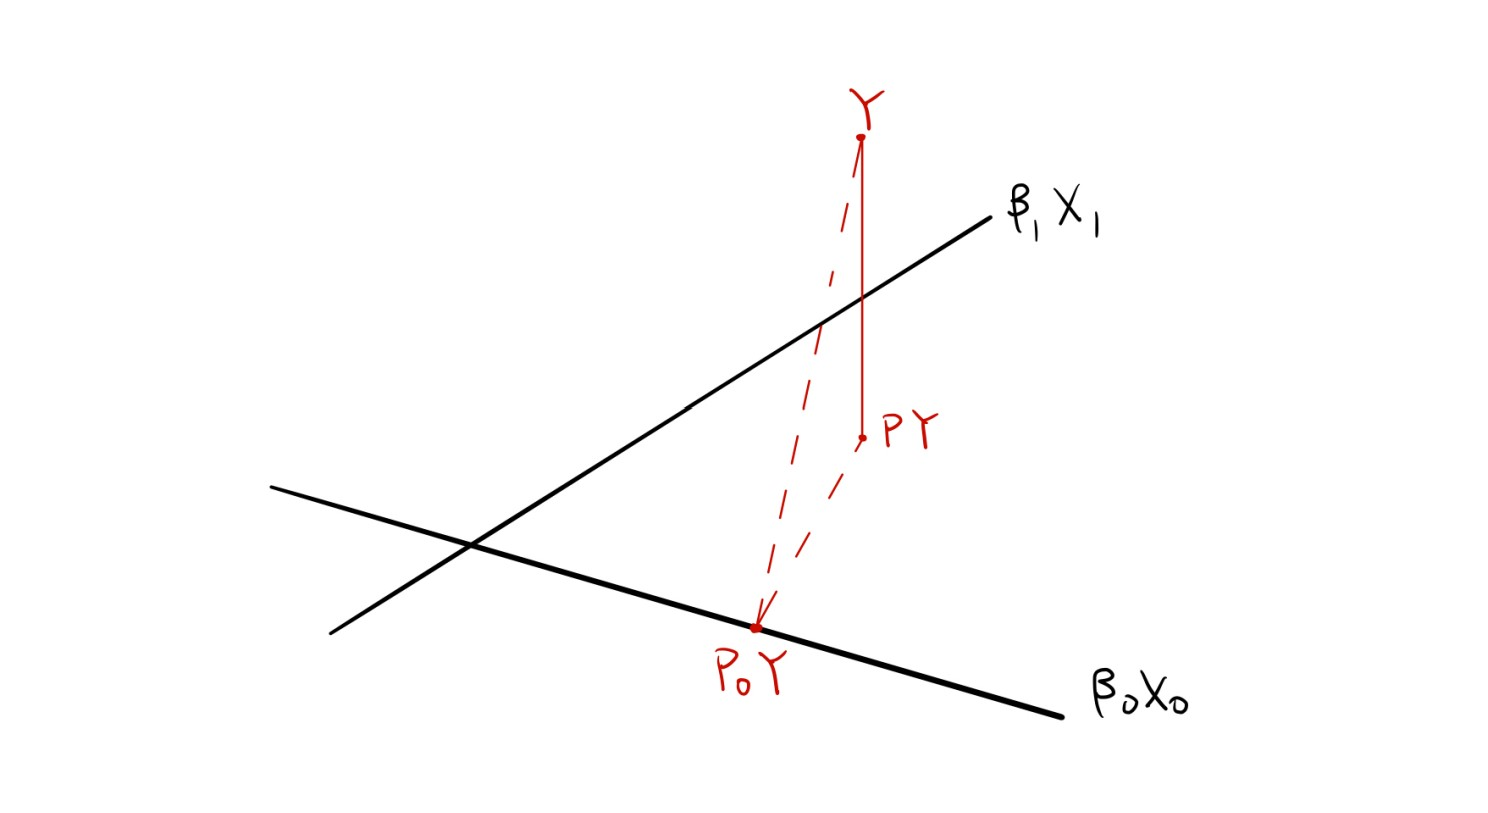
\includegraphics{img/Screenshot1.jpg}
		\caption{Nested model projections}
		\label{nested model projections}
		
	\end{figure}

	\begin{exer}[Simple linear regression]{exer:2}
		
		
	\end{exer}

	\subsection{Exact inference for the normal linear model}
	\label{exact inference}
	Besides motivating the OLS problem (\ref{defn:OLS}) as finding the MLE of $ \boldsymbol{\beta} $ in the normal linear model, the rest of highlighted (\ref{imp:normal model}) was entirely algebraic. \\
	In this section, we discuss statistical properties of the OLS estinator and how to use it to make exact inference under the normal linear model in highlighted (\ref{imp:normal linear model}).
	
	\subsubsection{Multivariate normal and related distributions}
	\begin{defn}[Multivariate normal distribution]{defn:MVN}
		A d-dimensional random vector $ \boldsymbol{Z} $ is said to follow the \hl{multivariate normal} distribution with mean $ \boldsymbol{\mu} \in \real^d $ and covariance matrix $ \boldsymbol{\sum} \in \real^{d \times d} $, written as $ \boldsymbol{Z} \sim N_d(\boldsymbol{\mu}, \boldsymbol{\sum}) $, if its probability density function is given by
		\[f(\boldsymbol{z}) = \frac{1}{(2\pi)^{d/2}|\boldsymbol{\sum}|^{1/2}} = e^{-(\boldsymbol{z} - \boldsymbol{\mu})^T\boldsymbol{\Sigma}^{-1}(\boldsymbol{z} - \boldsymbol{\mu})/2}  \]
	\end{defn}

	\begin{lem}[Important properties of the multivariate normal distribution]{lem:MVN}
		\begin{enumerate}[(i)]
			\item if $ \bZ \sim N_d(\bmu, \boldsymbol{\sum}) $, then for any fixed matrix $ \boldsymbol{A}\in \real^{k \times d} $ and vector $ \vec{b} \in \real^k $, $ \boldsymbol{A} \bZ + \vec{b} \sim N_k(\boldsymbol{A}\bmu + \vec{b}, \boldsymbol{A} \boldsymbol{\sum} \boldsymbol{A}^T) $.
			
			\item If $ \bZ_1 $ and $ \bZ_2 $ are two random vectors and $ \begin{bmatrix}
				 \bZ_1  \\  \bZ_2 
			\end{bmatrix} $ follows a multivariate normal distribution, then $ \bZ_1 \indep \bZ_2 $ iff $ Cov(\bZ_1, \bZ_2) = 0 $
		
			\item let $ \bZ \sim N_d(0, \boldsymbol{I}) $. Then 
			\[||\bZ||^2 = \sum_{i = 1}^{d}Z_i^2 \sim \chi_d^2\]
			follows the chi-squared distribution with d degrees of freedom. The following result will be useful for us. \\
			\textcolor{red}{Suppose $ \boldsymbol{P} \in \real^{d \times d} $ and $ rank(\bP) = r $, then $ ||\bP \bZ||^2 \sim \chi_r^2 $.}
		\end{enumerate}
		
	\end{lem}

	\begin{exer}[Prove last result]{exer:3}
		Confused what the exercise is, also the working out included in zhao's notes
	\end{exer}

	\subsubsection{Distribution of $ \hbb $ and $ \hat{\sigma}^2 $}
	Since $ \hbb = (\bX^T \bX)^{-1} \bX^T\bY $ is a linear transformation of Y, it has MVN distribution conditional on $ \bX $:
	\[\hbb \sim N((\bX^T \bX)^{-1} \bX^T \bmu, (\bX^T \bX)^{-1} \bX^T \sigma^2 \boldsymbol{I}_n \bX (\bX^T \bX)^{-1} \\ 
	= N(\beta, \sigma^2(\bX^T\bX)^{-1})
	\] 
	
	The estimator $ \hat{\sigma}^2 $ of the noise variance $ \sigma^2 $ can be written as 
	\[\hat{\sigma}^2 = \frac{1}{n-p} ||\bY - \bX \hbb||^2 = \frac{1}{n-p}||(\boldsymbol{I}_n - \bH)\bY||^2\]
	
	Because $ (\boldsymbol{I}_n - \bH)  $ is also a projection matrix, this implies that 
	
	\[\hat{\sigma}^2 | \bX \sim \frac{\sigma^2}{n-p} \chi_{n-p}^2\]
	
	This shows $ \mathbb{E}[\hat{\sigma}^2] = \sigma^2 $, hence $ \hat{\sigma}^2 $ is unbiased.
	
	\begin{exer}{exer:4}
		Show $ \hbb $ and $ \hat{\sigma}^2 $ are still unbiased without the normality assumption, that is, by only assuming $ \epsilon $ given $ \bX $ has mean $ \boldsymbol{0} $ and covariance matrix $ \sigma^2 \boldsymbol{I}_n $. \\
	
	\end{exer}
	
	Finally, $ \hbb $ and $ \hat{\sigma}^2 $ are independent under the normal linear model, because, given $ \bX $, $ (\bX^TX)^{-1}\bX^T \bY $ and $ (\boldsymbol{I}_n - \bH)\bY $ are jointly normal and 
	
	\[Cov((\boldsymbol{I}_n - \bH)\bY, (\bX^TX)^{-1}\bX^T \bY) = (\boldsymbol{I}_n - \bH) \sigma^2 \boldsymbol{I}_n \bX (\bX^T \bX)^{-1} = 0\]
	
	\subsubsection{Confidence sets}
	For the rest of this section, we view $ \bX $ as fixed (in other words, the inference is conditional on $ \bX $) (\textcolor{red}{What does this mean?}).
	The key to exact inference is to find \hl{pivotal quantities} whose distribution does not depend on unknown parameters. For example,
	
	\begin{imp}{imp:pivotal}
 		$\frac{(n-p)\hat{\sigma}^2}{\sigma^2} \sim \chi_{n-p}^2 $
	\end{imp}

	Is pivotal, but 
	
	\begin{imp}{imp:not pivotal}
		$ \hbb - \boldsymbol{\beta} \sim N(0, \sigma^2(\bX^T \bX)^{-1}) $
	\end{imp}

	is not pivotal because the distribution depends on $ \sigma^2 $. Instead, we can use the following pivotal quantity:
	
	\begin{imp}{imp:pivotal 2}
		$ \frac{\hbb - \boldsymbol{\beta}}{\hat{\sigma}} \sim \frac{N(\boldsymbol{0}, (\bX^T \bX)^{-1})}{\sqrt{\chi_{n-p}^2/(n-p)}} $
	\end{imp}
	
	Element-wise, we have
	
	\begin{imp}{imp:pivotal 3}
		$\frac{\hat{\beta}_j - \beta_j}{\hat{\sigma}} \sim \frac{N(0, (\bX^T \bX)_{jj}^{-1})}{\sqrt{\chi_{n-p}^2/(n-p)}} = \sqrt{(\bX^T \bX)_{jj}^{-1}} \times t_{n-p}, \quad j = 1, ..., p$
	\end{imp}

	By using Highlight (\ref{imp:pivotal 3}), we can immediately construct a $ (1-\alpha) $ confidence interval for $ \beta_j $:
	
	\[CI_j(\alpha) = [\hat{\beta}_j - \hat{\sigma} \sqrt{(\bX^T \bX)_{jj}^{-1}} t_{n-p}(\alpha/2), \hat{\beta}_j + \hat{\sigma} \sqrt{(\bX^T \bX)_{jj}^{-1}} t_{n-p}(\alpha/2)]\]
	
	Where $ t_{n-p}(\alpha/2) $ is the upper $ (\alpha/2) $-quantile of $ t_{n-p} $. 
	
	\begin{defn}[$ (1-\alpha) $ confidence interval for $ \beta_j $: $ CI_j(\alpha) $]{defn:Confidence interval}
		$ \mathbb{P}(\beta_j \in CI_j(\alpha)) = 1-\alpha $
		
	\end{defn}
	

	To construct a confidence region for the p-dimensional vector $ \beta $, a simple approach is to take the product of univariate confidence intervals $ \prod_{j = 1}^{p} CI_j(\alpha/p) $. \textcolor{blue}{(Exercise: Show that this set covers $ \boldsymbol{\beta} $ with probability at least $ 1-\alpha $)}\\
	
	However, this product set is usually quite \hl{conservative} \textcolor{pink}{What does conservative mean?} because it does not take into account the dependence between the entries of $ \hbb $. A better solution is to use the following pivotal quantity:
	\begin{imp}[F distribution]{imp:F distribution}
		$\frac{(\hbb - \boldsymbol{\beta})^T(\bX^T \bX)(\hbb - \boldsymbol{\beta})}{p \hat{\sigma}^2} \sim F_{p, n-p}$
	\end{imp}

	So the following ellipsoid is a $ (1-\alpha) $ confidence region of $ \boldsymbol{\beta} $:
	
	\[CI(\alpha) = {\boldsymbol{\beta}\in \real^p | \frac{(\hbb - \boldsymbol{\beta})^T(\bX^T \bX)(\hbb - \boldsymbol{\beta})}{p \hat{\sigma}^2} \leq F_{p, n-p}(\alpha)}\]
	
	where $ F_{p, n-p}(\alpha) $ is the upper $ \alpha $-quantile of $ F_{p, n-p} $.
	
	\begin{exer}{exer:5}
		Use (\ref{imp:pivotal}) to construct a $ (1-\alpha) $-confidence interval for $ \sigma^2 $.
	\end{exer}
	\begin{exer}{exer:6}
		let $ (\bX^*, Y^*) \in \real^p \times \real $ be a new observation of the normal linear model. That is, suppose $ Y^* =  $
	\end{exer}

	\subsubsection{Hypothesis tests and analysis of variance}
	
	By using the duality between hypothesis testing and confidence interval, we can easily construct level-$ \alpha $ tests for 
	\[H_0: \beta_j = 0 \quad vs. \quad H1: \beta_j \neq 0 and H_0: \boldsymbol{\beta} = \boldsymbol{0} \quad vs. \quad H_1: \boldsymbol{\beta} \neq \boldsymbol{0}\]
	
	That is, we reject $ \beta_j = 0 $ if $ 0 \notin CI_j(\alpha) $ and reject $ \boldsymbol{\beta} = \boldsymbol{0} $ if $ \boldsymbol{0 \notin CI(\alpha)} $
	
	More generally, we may be interested in comparing nested linear models. As before, consider the following partition 
	\[\bX = (\bX_0 \bX_1) and \boldsymbol{\beta} \begin{bmatrix}
		\boldsymbol{\beta}_0 \\ \boldsymbol{\beta}_1
	\end{bmatrix}\]

	where $ \bX_0 \in \real^{n \times p_0} $ and $ \beta_0 \in \real^{p_0} $.\\
	We are interested in comparing the full model $ \bmu = \bX \boldsymbol{\beta} $ with the submodel $ \bmu = \bX_0 \boldsymbol{\beta}_0 $, which amounts to testing $ H_0: \boldsymbol{\beta}_1 = 0 \quad vs. \quad H_1: \boldsymbol{\beta}_1 \neq 0 $.\\
	
	The \hl{(generalised) likelihood ratio statistic} is given by
	\[\frac{sup_{\boldsymbol{\beta}\in \real^p} L(\boldsymbol{\beta}, \sigma^2)}{sup_{\boldsymbol{\beta}_0 \in \real^{p_0}, \boldsymbol{\beta}_1 = 0} L(\boldsymbol{\beta}, \sigma^2)}  =  exp\{\frac{n}{2} + \frac{n}{2} \frac{||(\bP - \bP_0)\bY||^2}{||(\boldsymbol{I}-\bP)\bY||^2}\}\]
	
	\begin{exer}[Prove The above equality]{exer:ineq}
		
	\end{exer}
	
	Thus, the likelihood ratio test rejects $ H_0 $ if $ \frac{||(\bP - \bP_0)\bY||^2}{||(\boldsymbol{I}-\bP)\bY||^2} $ is large.\\
	Note that $ ||(\boldsymbol{I}-\bP)\bY||^2 $ is the residual sum of squares (RSS) of the full model, while $ ||(\bP - \bP_0)\bY||^2 $ is the reduction of RSS when we enlarge the submodel to the full model. This ratio has obvious geometric interpretations; see Figure (\ref{nested model projections}) \\
	
	To determine the critical value, we need to derive the distribution of the test statistic under $ H_0: \boldsymbol{\beta}_1 = 0 $. Under this null hypothesis, $ \bY = \bX \boldsymbol{\beta} + \boldsymbol{\epsilon} = \bX_0 \boldsymbol{\beta}_0 + \boldsymbol{\epsilon}$.\\
	Therefore, 
	\[\frac{||(\bP - \bP_0)\bY||^2}{||(\boldsymbol{I}-\bP)\bY||^2} = \frac{||(\bP - \bP_0)\boldsymbol{\epsilon}||^2}{||(\boldsymbol{I}-\bP)\boldsymbol{\epsilon}||^2}\]
	
	Because $ \epsilon $ follows a multivariate normal distribution (\textcolor{red}{Do we assume the model is normal here? why?}) and 
	\[Cov((\bP-\bP_0)\boldsymbol{\epsilon}, (\boldsymbol{I}-\bP) \boldsymbol{\epsilon}) = (\bP-\bP_0)\sigma^2 \boldsymbol{I}(\boldsymbol{I}-\bP) = 0\]
	
	This implies $ (\bP - \bP_0)\epsilon \indep (\boldsymbol{I}-P)\epsilon $ by Lemma (\ref{lem:MVN})
	
	Because $ \bP - \bP_0 $ and $ \boldsymbol{I} - \bP $ are projection matrices, $ ||(\bP - \bP_0)\epsilon||^2 \sim \chi_{p-p_0}^2 $ and $ ||(\boldsymbol{I}-P)\epsilon||^2 \sim \chi_{n-p}^2 $.\\
	Therefore,
	\[F = \frac{||(\bP - \bP_0)\bY||^2/(p-p_0)}{||(\boldsymbol{I}-\bP)\bY||^2/n-p} \sim F_{p-p_0, n-p} \quad under \quad H_0\]
	Hence the level - $ \alpha $ likelihood ratio test rejects $ H_0 $ when $ f > F_{p-p_0, n-p}(\alpha) $.
	
	\begin{exer}[Show that the t-test and F-test for $ H_0: \beta_j = 0 $ vs. $ H_1: \beta_j > 0 $ are equivalent]{exer:f and t test same}
		
	\end{exer}

	\subsection{Linear conditional expectation model}
	
	\begin{imp}[Assumptions]{imp:linear model assumptions recap}
		As discussed in Section (\ref{the normal linear model section}), the normal linear model contains three assumptions:
		\begin{enumerate}[(i)]
			\item The conditional expectation follows a linear model $ \bmu = \bX \boldsymbol{\beta} $
			\item the noise $ \boldsymbol{\epsilon} $ is independent of $ \bX $
			\item the noise $ \boldsymbol{\epsilon} \sim N(\boldsymbol{0}, \sigma^2 \boldsymbol{I}_n) $
		\end{enumerate}
		
		The last two distributional assumptions play an essential role in the exact statistical inference discussed in Section (\ref{exact inference}) but are often too restrictive in applications. Next, we briefly discuss relaxations of these assumptions.
	\end{imp}
	
	\subsubsection{Generalised least squares}
	One possible relaxation is to assume $ \boldsymbol{\epsilon} $ follows a non-isotropic normal distribution:
	\[\bY = \bX \boldsymbol{\beta} + \boldsymbol{\epsilon}, \quad \boldsymbol{\epsilon} | \bX \sim N(0, \sigma^2 \boldsymbol{\Sigma})\]
	where $ \sigma^2 \in \real $ is unknown and $ \boldsymbol{\Sigma} \in \real^{n \times n} $ is known positive-definite matrix that may depend on $ \bX $. \\
	
	Theoretical results in Sections (\ref{section:Ordinary least squares and its geometry} and (\ref{exact inference}) can be easily extended to this model by using the transformation $ \bX \rightarrow \boldsymbol{\Sigma}^{-1/2} \bX $ and $ \bY \rightarrow \boldsymbol{\Sigma}^{-1/2} \bY $.\\
	The maximum likelihood estimator for $ \boldsymbol{\beta} $ in this model is given by the \hl{generalised least squares (GLS)} estimator:
	\[\hbb_{GLS} = (\bX^T \boldsymbol{\Sigma}^{-1}\bX)^{-1}\bX^T \boldsymbol{\Sigma}^{-1}\bY\]
	
	\begin{exer}[Derive the above formula for $ \hbb_{GLS} $ from the definitions. Then derive it again using the formula for $ \hbb_{OLS} $.]{exer:derive GLS}
		
	\end{exer}

	An important special case of GLS is the \hl{weighted least squares (WLS)}. 
	\begin{defn}[weighted least squares(WLS)]{defn:WLS}
		Given a vector of weights $ \boldsymbol{\omega} = (\omega_1, ..., \omega_n) $, the WLS estimator is given by:
		\[\hbb_{WLS} = arg \: min_{\boldsymbol{\beta}} \sum_{i = 1}^{n} \omega_i(Y_i - \bX_i^T \boldsymbol{\beta})^2 \]
		
		This is equivalent to choosing $ \boldsymbol{\Sigma} = diag(\omega_1^{-1}, ..., \omega_n^{-1}) $ in GLS
	\end{defn}

	\subsubsection{Heteroscedasticity}
	Consider the followig less restrictive linear model:
	\begin{imp}[less restrictive linear model]{imp:LR linear model}
		\[y_i = \bX_i^T \boldsymbol{\beta} + \epsilon_i, \; i = 1, ..., n,\]
		where
		\begin{enumerate}
			\item $ (\epsilon_i, \bX_i), \; i = 1, ..., n $ are independent and identically distribution (IID)
			\item $ \mathbb{E}(\epsilon_i | \bX_i) = 0 $
			\item $ Var(\epsilon_i | \bX_i) = \sigma^2(\bX_i) $
		\end{enumerate}
	\end{imp}

	Compared to the classical normal linear model in highlight (\ref{imp:normal linear model}), highlight (\ref{imp:LR linear model}) no longer assumes $ \epsilon_i \indep \bX_i $, the distribution of $ \epsilon_i $ is normal, or the variance of $ \epsilon_i $ is a constant.\\
	When $ \sigma^2(\bX_i) = \sigma^2 $ is a constant, we say the noise is \hl{homoscedastic}; otherwise, we say the noise is \hl{heteroscedastic}.\\
	
	Due to the lack of distributional assumptions, exact statistical inference is no longer possible. However, we can rely on asymptotic arguments:
	\[\sqrt{n}(\hbb - \boldsymbol{\beta}) = \sqrt{n} \{(\bX^T\bX)^{-1}\bX^T \bY - \boldsymbol{\beta}\} \\
	= \sqrt{n} \{(\bX^T\bX)^{-1}\bX^T (\bX \boldsymbol{\beta} + \boldsymbol{\epsilon}) - \boldsymbol{\beta}\}\\
	= \sqrt{n}(\bX^T\bX)^{-1}\bX^T \boldsymbol{\epsilon}\\
	= (\frac{1}{n}\sum_{i = 1}^{n} \bX_i \bX_i^T)^{-1}(\frac{1}{\sqrt{n}}\sum_{i = 1}^{n} \bX_i \epsilon_i)
	\]
	Under suitable regularity conditions, the first term converges in probability to $ \boldsymbol{\Sigma}_X = \mathbb{E}[\bX_i \bX_i^T] $ by the weak law of large numbers. Therefore, by \textcolor{blue}{Slutsky's lemma} (\textcolor{red}{What is the Slutsky's lemma?}), 
	\begin{imp}{imp:by slutsky}
		$\sqrt{n}(\hbb - \boldsymbol{\beta}) \stackrel{d}{\rightarrow} N(\boldsymbol{0}, \bSigma_X^{-1} \boldsymbol{\Omega} \bSigma_X^{-1} ), \; as n \rightarrow \infty$
	\end{imp}

	\begin{defn}[Sandwich variance or inverse Godambe information]
		The form of matrix $ \bSigma_X^{-1} \boldsymbol{\Omega} \bSigma_X^{-1} $ is common in misspecified maximum likelihood and is often called the sandwich variance or the inverse Godambe information
	\end{defn}

	When the noise is homoscedastic, i.e. $ \sigma^2(\bX_i) = \sigma^2 $, this reduces to 
	\[\sqrt{n}(\hbb - \bbeta) \stackrel{d}{\rightarrow} N(0, \sigma^2 \bSigma_X^{-1})\]
	which is consistent with the exact distribution in highlight (\ref{imp:not pivotal}) obtained under normality.\\
	Equation in highlight (\ref{imp:by slutsky}) is not an (asymptotic) pivotal quantity yet becase the distribution depends on $ \bSigma $ and $ \Omega $. These unknown quantities can be estimated by 
	\[\hat{\bSigma}_X = \frac{1}{n}\sum_{i = 1}^{n} \bX_i \bX_i^T \text{ and } \hat{\boldsymbol{\Omega}} = \frac{1}{n}\sum_{i = 1}^{n} \bX_i \bX_i^T e_i^2\]
	
	Under suitable regularity conditions, they converge to $ \bSigma_X $ and $ \boldsymbol{\Omega} $ in probability.\\
	By Slutsky's lemma, 
	\[\sqrt{n} \hat{\bSigma}_X \hat{\boldsymbol{\Omega}}^{-1/2}(\hbb - \bbeta) \stackrel{d}{\rightarrow} N(0, \boldsymbol{I}_p) \text{, as } n \rightarrow \infty\]
	
	It is then straightforward to construct confidence intervals or hypothesis tests for $ \boldsymbol{\beta} $.
	
	\subsubsection{Misspecified linear models}
	One may further question the validity of the linear model $ \boldsymbol{\mu} = \bX\beta $ itself.  \\
	To emphasize that the linear model could be misspecified, we sometimes call $ \boldsymbol{\mu} = \bX \beta $ a \hl{linear working model}. Consider the following setting:
	\begin{imp}[Setting]{imp:setting}
		$ Y_i = g(\bX_i) + \epsilon_i $, where $ (\bX_i, \epsilon_i) $ are IID, $ \epsilon_i \indep \bX_i $, $ \mathbb{E}(\epsilon_i) = 0, \; i = 1, ..., n $
	\end{imp}
	
	In \hl{nonparametric regression}, the goal is to estimate the regression function $ g(\cdot) $. A \hl{parametric model} such as the linear model assumes $ g(\cdot) $ belongs to a class of functions $ {g(\cdot;\bbeta)| \boldsymbol{\beta} \in \real^p} $ that is indexed by some finite-dimensional parameter $ \bbeta $. Here, our interest is to understand how the linear working model behaves when the truth is highlight (\ref{imp:setting}).\\
	
	Recall that the OLS estimator $ \hbb $ minimises $ \sum_{i = 1}^{n} (Y_i - \bX_i^T \bbeta) $. Therefore, it is expected that, as $ n \rightarrow \infty $, $ \hbb $ will converge to 
	\begin{align}
		\bbeta_{OLS} & = arg \; min_{\bbeta} \mathbb{E}\{(Y_i - \bX_i^T \bbeta)^2\} \\
	& = arg \; min_{\bbeta} \mathbb{E}\{(g(\bX_i) - \bX_i^T \bbeta + \epsilon_i)^2\}\\
	& = arg \; min_{\bbeta} \mathbb{E}\{(g(\bX_i) - \bX_i^T \bbeta)^2\} + \underbrace{\mathbb{E}\{(g(\bX_i - \bX_i^T \bbeta)\epsilon_i)\}}_{= 0} + \underbrace{\mathbb{E}(\epsilon_i^2)}_\text{$ = $ constant}\\
	& = arg \; min_{\bbeta} \mathbb{E}\{(g(\bX_i) - \bX_i^T \bbeta)^2\}
	\end{align}
	
	Therefore, $ \bX_i^T \bbeta_{OLS} $ may be viewed as the projection of $ g(\bX_i) $ onto the space of linear functions of $ \bX_i $.\\
	
	We make two remarks on misspecified linear models. \\
	First, the "true" value of the parameter $ \bbeta_{OLS} $ depends on the distribution of $ \bX_i $; see Figure () for an illustration.\\
	Second, the definition of the population regression coefficient $ \bbeta $ also generally depends on the estimator we use. For example, the \hl{least absolute deviation (LAD)} estimator:
	\[\hbb_{LAD} = arg \; min_{\bbeta} \sum_{i = 1}^{n}|Y_i - \bX_i^T \bbeta|\]
	
	does not generally converge to $ \bbeta_{OLS} $, unless the linear model is correctly specified (i.e. $ g(\boldsymbol{x}) $ is indeed linear in $ \boldsymbol{x} $).
	
	%%%%%%%%%%%%%%%%%%%%%%%%%%
	%insert figure 2.2 in notes: on true value of beta_OLS
	%%%%%%%%%%%%%%%%%%%%%%%%%%
	
	\subsubsection{Omitted-variables bias and simpson's paradox}
	Misspecified models may also arise if some \hl{covariates} are omitted in the regression.\\
	Consider two linear models:
	\begin{imp}{imp:tow linear models}
		Model 1: $ Y_i = \bX_i^T \bbeta + \epsilon_i $	\\	
		Model 2: $ Y_i = \bX_i^T \bbeta^*+ \bZ_i^T \boldsymbol{\gamma}^* + \epsilon_i^* $
	\end{imp}

	In general, $ \bbeta \neq \bbeta^* $, a phenomenon often regerred to as the \hl{ommoted-variable bias}
	
	
	\begin{exer}[Show that $ \bbeta = \bbeta^* $ if $ \bX_i \indep \bZ_i $.][exer:2.12]
		
	\end{exer}
	
	In its extreme form, ommited-variable bias is known as Simpson's paradox, which was initially discovered by K.Pearson and U.Yule. One of the best-known examples is the 1973 Berkeley admission data; see Figure (\ref{img:Berkeley admission data}). Overall, men appear to be more likely to be admitted than women. However, if we look at the department-level statistics, in most cases women have a higher admission rate. \\
	This apparent paradox can be explained by the observation that there appear to be more men applications to departments with a higher admission rate. Whether this is also a kind of "gender bias" is another matter of debate.\\
	Fundamentally, the reason behind Simpson's paradox is that a regression coefficient only measures (conditional) association and does not necessarily indicate causation. A rigorous discourse on causation is beyond the scope of this course.
	
	\begin{figure}[h]
		\centering
		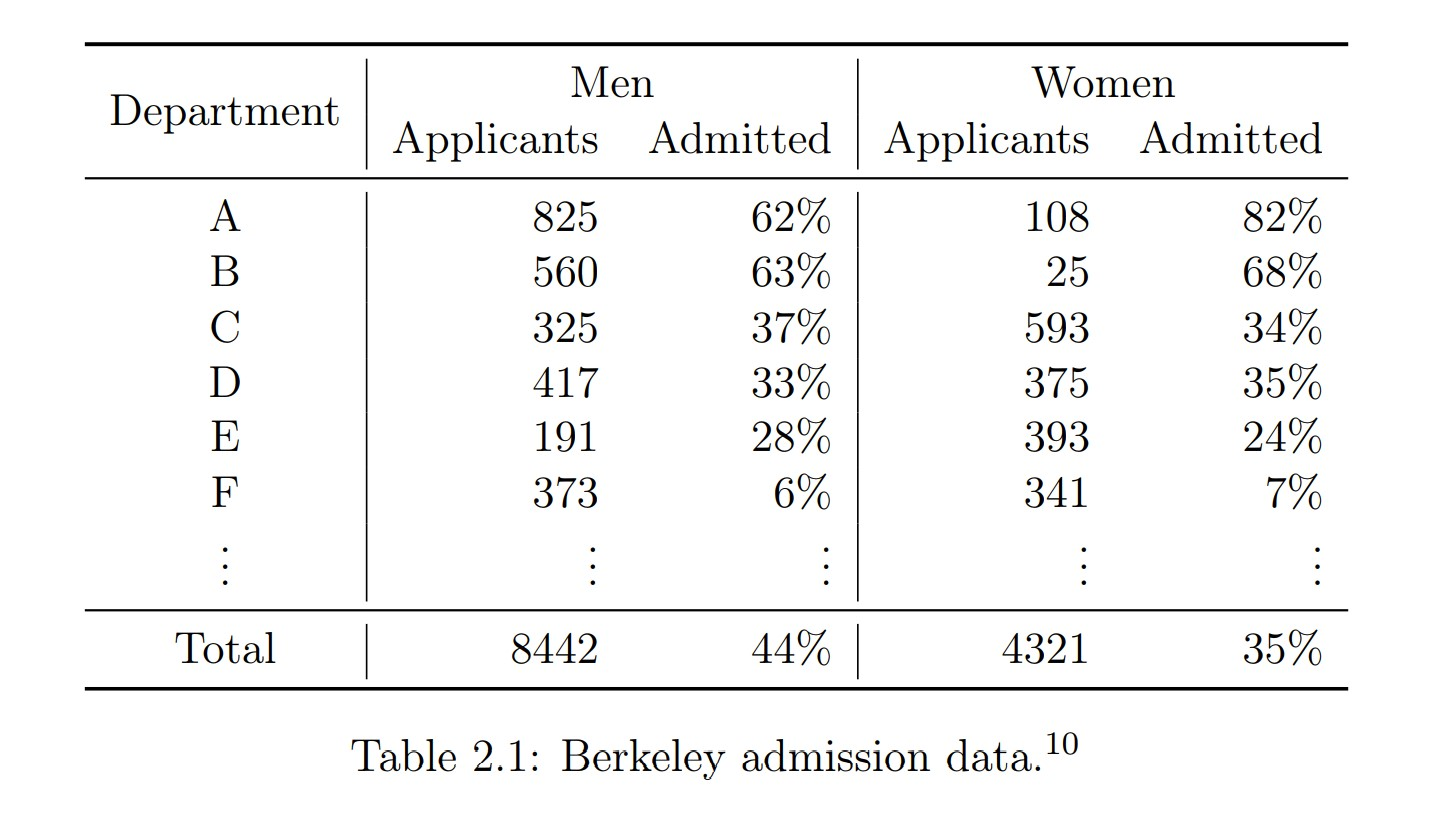
\includegraphics{img/Screenshot2.jpg}
		\caption{Berkely admission data}
		\label{img:Berkeley admission data}
		
	\end{figure}

	\subsection{Model diagnostics and model selection}
	Although the normal linear model makes several restrictive assumptions, it remains the default choice for many applications used due to its simplicity. In practice, a common task is to select a linear working model according to one or some of the following criteria:
	\begin{enumerate}[(i)]
		\item Does the model appreas to provide a good fit to the observed data?
		\item How large is the model's prediction error?
		\item How likely is the true model covered, assuming the data are indeed generated from it?
		\item How interpretable is the model?
	\end{enumerate}
	This section will provide some theoretical insights for the first three considerations.
	
	\subsubsection{Linear model diagnostics}
	One nice thing about making restrictive assumptions is that we can often check them empirically. Here we provide some useful diagnostic quantities and plots for the normal linear model.\\
	To measure how well the linear model fits the observed data, a widely used value is the coefficient of determination, defined as
	\[R^2 = \frac{||\hbmu - \bar{Y}\boldsymbol{1}||^2}{||\bY - \bar{Y}\boldsymbol{1}}||^2 = 1-\frac{||\bY - \hbmu||^2}{||\bY - \bar{Y}\boldsymbol{1}}||^2\]
	where $ \bar{Y} = \sum_{i = 1}^{n} Y_i / n $.\\
	In words, $ R^2 $ is a measure of the proportion of variance of $ Y_i $ that can be explained by the linear model. A common mistake in practice is to interpret the absolute value of $ R^2 $ out of context, which depends crucially on the level of noise in the observations. So a lienar model with $ R^2 = 1\% $ is not necessarily a poor model.\\
	The \hl{leverage} of the ith obervation is defined as $ H_{ii} $, the ith diagonal element of the hat matrix. Recall that the fitted value for $ Y_i $ is 
	\[\hat{\mu}_i = (\bH \bY)_i = H_{ii} Y_i + \sum_{k \neq i} H_{ik}Y_k\]
	So the leverage $ H_ii $ is how much the observed value $ Y_i $ determines the fitted value $ \hat{\mu}_i $.\\
	Another motivation for leverage is the following result (recall $ \boldsymbol{R} = \bY - \hbmu $ is the vector of residuals)
	\begin{imp}{imp:motivation for leverage}
		$ Var(R_i | \bX) = \sigma^2(1-H_{ii}) $
	\end{imp}
	So the residual $ R_i $ is close to 0 if the leverage $ H_{ii} $ is close to 1.
	
	\begin{exer}[Prove highlight (\ref{imp:motivation for leverage})]{exer:2.13}
		
	\end{exer}
	
	Next we describe the \hl{diagnostic plots} produced by the $ R $ function $ plot.lm $ by default \textcolor{red}{can't find plot.lm}.\\
	The first is the \hl{residual vs. fitted} plot, which plots the studentized residual $ \tilde{R}_i $ against the predicted value $ \hat{\mu}_i $. We can visually assess the assumption $ \mathbb{E}(\epsilon_i|\bX_i) = 0 $, by checking if there is any obvious trend (e.g. a quadratic trend) in the plot.\\
	The second is the \hl{quantile-quantile (Q-Q)} plot, which is used to visually check normality of the noise $ \epsilon_i $. Motivated by highlight (\ref{imp:motivation for leverage}), the \hl{studentized} or \hl{stadardised residual} of the ith observation is defined as 
	\[\tilde{R}_i = \frac{R_i}{\hat{\sigma} \sqrt{1-H_{ii}}}\]

	If the normal linear model is correct, $ \tilde{R}_i $ should be close to $ \epsilon_i/\sigma $, which follows a standard normal distribution.\\
	We may check this assumption by plotting the sample quantiles of $ (\tilde{R}_1, ..., \tilde{R}_n) $ against the theoretical quantiles of $ N(0, 1) $; see Figure (\ref{img:qqplot}) for an illustration.
	
	\begin{figure}[h]
		\centering
		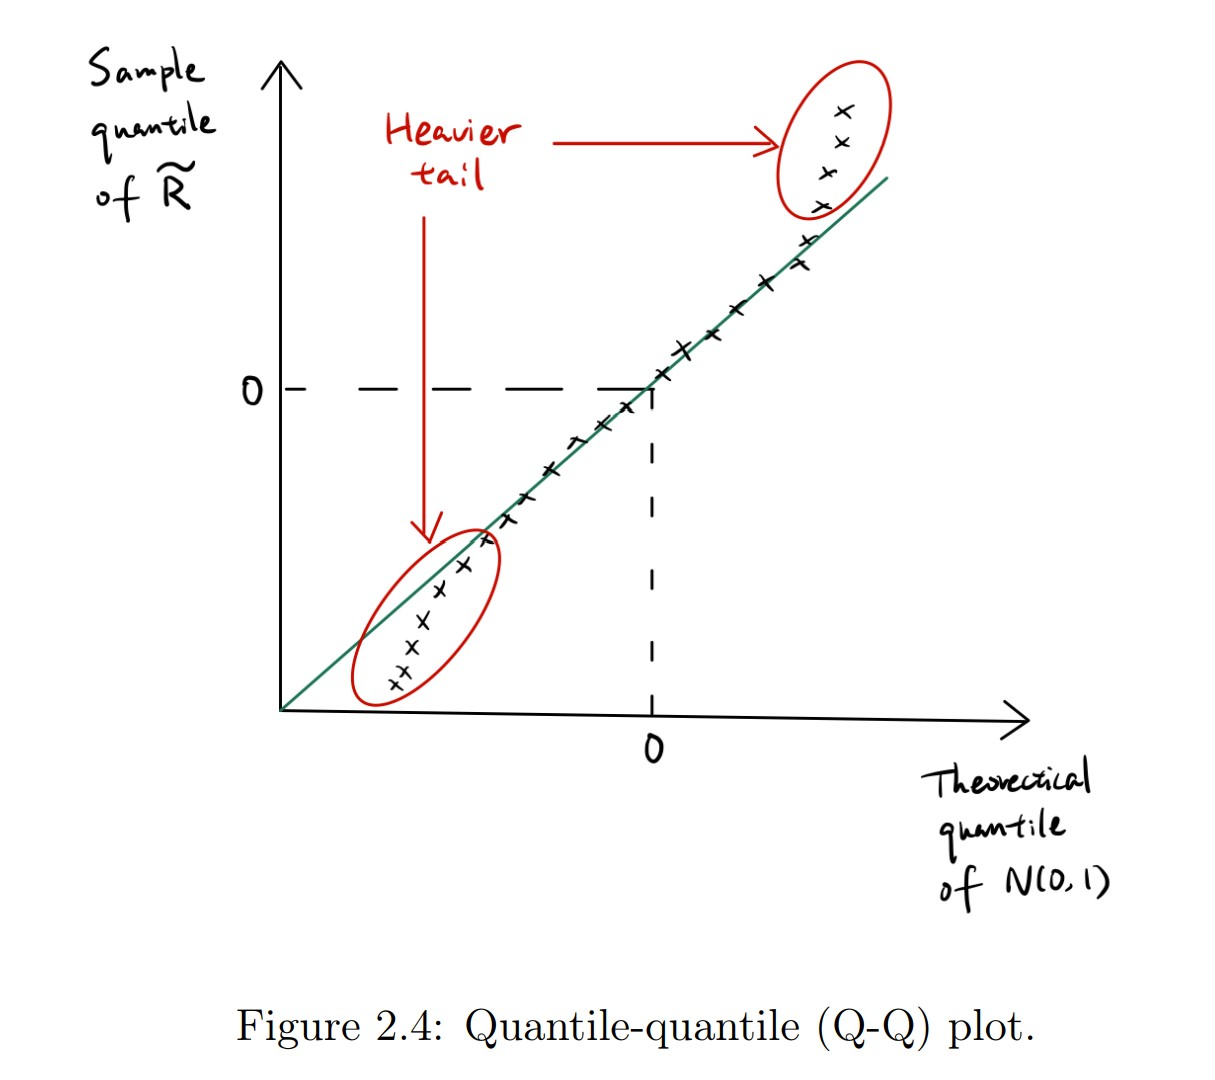
\includegraphics{img/Screenshot3.jpg}
		\caption{Quantile-quantile (Q-Q) plot}
		\label{img:qqplot}
		
	\end{figure}


	\begin{exer}[In the normal linear model, show that $ \tilde{R}_i \sim t_{n-p-1} $ if we replace $ \hat{\sigma} $ in the definition of $ \tilde{R}_i $ by $ \hat{\sigma}_{(-i)} $, which is the estimator of $ \sigma $ using all observations besides $ (X_i, Y_i) $.]{exer:2.14}
		
	\end{exer}

	The third diagnostic plot is the \hl{scale-location} plot, which shows the square root of the absolute value of the standardized residual $ \sqrt{|\tilde{R}_i|} $ against the fitted value $\hat{\mu}_i$. This plot is used to check the homoscedasticity assumumption $ Var(\epsilon_i| \bX_i) = \sigma^2 $, under which $ \sqrt{|\tilde{R}_i|} $ should have an average value around 1.\\
	The fourth and final one is a plot of \hl{residuals vs. leverage}. More precisely, this plot shows $ \tilde{R}_i $ against $ H_{ii} $ and is used to identify outliers with a large leverage.\\
	We say an observation $ (\bX_i, Y_i) $ is an outlier if $ |R_i| $ is much larger than what is expected if $ \epsilon_i \sim N(0, \sigma^2) $. In other words, these observations differ substantially from model-predicted values. Especially of concern are outliers with a high leverage, because just one or a few of them can severely bias a regression model. \\
	Note that the definition of "outlier" depends on the model. It is not rare to have one observation that is not an outlier originally become an outlier when some other aparently outlying observations are removed. See Figure (\ref{img:outliers with high leverage}) for an illustration.
	
	\begin{figure}[h]
		\centering
		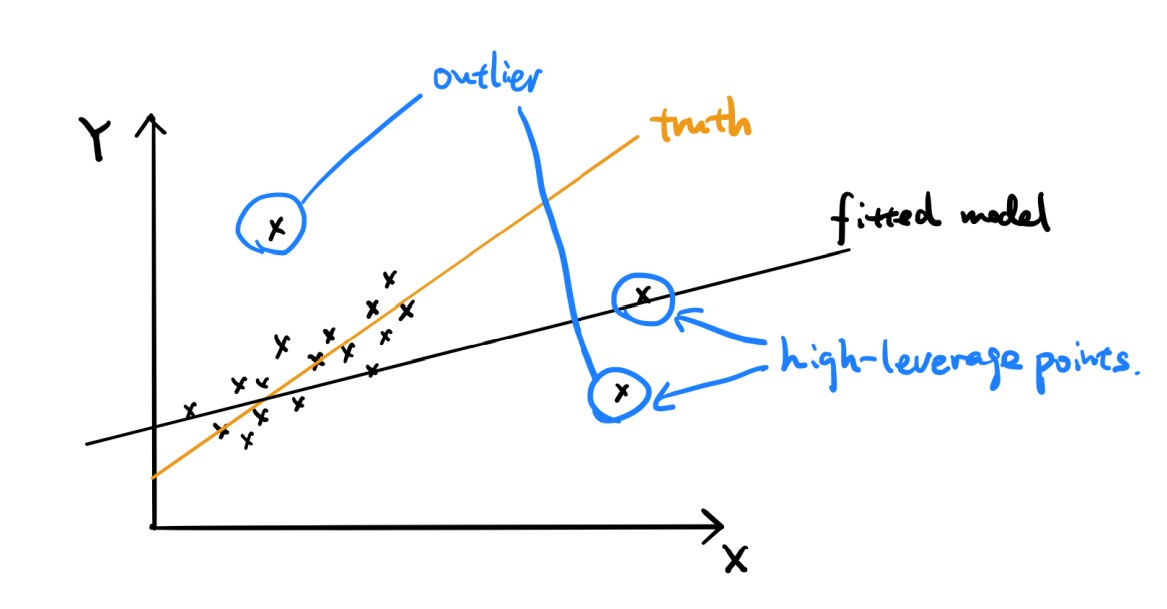
\includegraphics{img/Screenshot4.jpg}
		\caption{Outliers with a high leverage can severely bias a regression model}
		\label{img:outliers with high leverage}
	\end{figure}

	A useful quantity for outlier detection is Cook's distance:
	\begin{imp}[Cook's distance]{imp:cook's distance}
		$ D_i = \frac{||\bX(\hbb - \hbb_{(-i)})||^2}{p \hat{\sigma}^2} = \frac{1}{p}\frac{H_{ii}}{1-H_{ii}}\tilde{R}_i^2 $
	\end{imp}

	where $ \hbb_{(-i)} $ is the "leave-one-out" OLS estimator of $ \bbeta $ when $ (\bX_i,Y_i) $ is removed from the dataset. By definition, $ D_i $ is a standardized change of the fitted values when the ith observation is removed. \\
	Therefore, a large value of $ D_i $ indicates that the ith observation have a large influence on the fitted values. Some clever algebra produces the formula in (\ref{imp:cook's distance}), so in order to compute


\end{document}